\section{Exercice 3}
Le but de cet exercice est de créer un client pouvant se connecter à un serveur web, lui envoyer une requête HTTP, et afficher sa réponse.\\

Le programme utilise trois arguments : le premier est le hostname du serveur, le deuxième le port sur lequel on souhaite se connecter, et le troisième la ressource que l'on souhaite récupérer.\\

La première étape est l'initialisation d'une socket connectée à l'aide de la fonction \emph{init\_stream\_client \_socket()} qui a été décrite dans l'exercice précédent. Une fois cette première étape effectuée, nous souhaitons créer et envoyer une requête HTTP au serveur. La création de la requête HTTP se fait à l'aide de la fonction \emph{create\_GET\_request()} définie dans \emph{http\_tools.c}.\\

\begin{lstlisting}
char* create_GET_request(const char* host, const char* res, const char* port) {
    char *buf = malloc(BUFFER_LEN);

    int status = snprintf(buf, BUFFER_LEN,
        "GET %s HTTP/1.1\r\n"
        "Host: %s:%s\r\n"
        "Connection: close\r\n"
        "Accept: text/html\r\n\r\n",
        res, host, port
    );

    if(status < 0) {
        free(buf);
        return NULL;
    }

    return buf;
}
\end{lstlisting}
\

La ligne \emph{Connection: close} a été spécifiée afin que l'appel système \emph{read()} qui sera utilisé par la suite puisse retourner 0 lorsqu'il n'y a plus rien à recevoir de la part du serveur. Par défaut, \emph{Connection: Keep-Alive} est utilisé ce qui empêche le dernier read de retourner car la connexion n'a pas été fermée.\\

Une fois la requête créée, on l'envoie à l'aide de \emph{send\_complete()} (similaire à \emph{sendto\_complete()}, mais utilisant \emph{send()} à la place de \emph{sendto()}). On récupère ensuite la réponse à l'aide de \emph{recv\_print()} définie dans \emph{socket\_tools.c} qui effectue des appels à \emph{read()} tant que la taille reçue n'est pas égale à 0 (0 étant retourné lorsqu'il n'y a plus rien à recevoir).\\

\begin{lstlisting}
int recv_print(int sockfd) {
    int recv_size;
    char buf[BUFFER_LEN];

    do {
        recv_size = read(sockfd, buf, BUFFER_LEN - 1);
        if (recv_size == -1) {
            perror("read");
            break;
        }

        if (recv_size != 0) {
            buf[recv_size] = '\0';
            printf("%s", buf);
        }
    } while(recv_size != 0);

    return recv_size;
}
\end{lstlisting}
\newpage

\subsection{Exemple d'exécution}
\begin{figure}[h!]
	\centering
	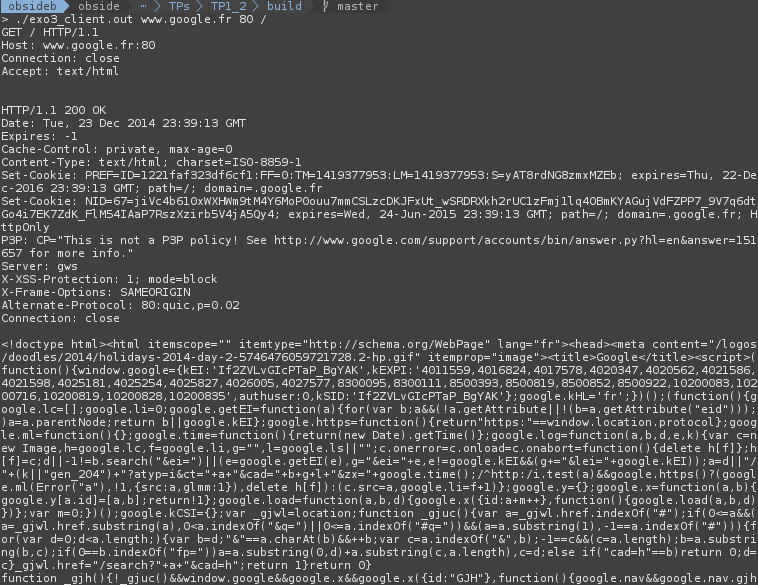
\includegraphics[width=1.0\textwidth]{screenshots/ex3.png}
	\caption{exo3\_client.out}
\end{figure}
